\documentclass[12pt,a4paper]{article}

\usepackage[UTF8]{ctex}
\usepackage[scale=0.8]{geometry}
\usepackage{latexsym,amsmath,amsfonts,amssymb,mathrsfs,bm}
\usepackage{abstract,appendix,titlesec,titletoc}
\usepackage{diagbox,booktabs,longtable,tabularx}
\usepackage[amsmath,thmmarks,hyperref]{ntheorem}
\usepackage{fancyhdr,indentfirst}
\usepackage[colorlinks=ture]{hyperref}
\usepackage{makeidx,cleveref}
\usepackage[sort&compress, numbers]{natbib}
\usepackage{graphicx,epsfig,subfig}
\usepackage{algorithm,algorithmicx,algpseudocode}
\usepackage{xcolor}

\linespread{1.3}
\setlength{\parskip}{0.5\baselineskip}

\theoremstyle{plain}
\newtheorem{definition}{定义}
\newtheorem{example}{例}
\newtheorem{theorem}{定理}
\newtheorem{lemma}{引理}
\newtheorem{corollary}{推论}
\newtheorem{remark}{注}
\newtheorem{proposition}{性质}

\newcommand{\Rnum}{\mathbb{R}}
\newcommand{\Cnum}{\mathbb{C}}
\newcommand{\Znum}{\mathbb{Z}}
\newcommand{\Nnum}{\mathbb{N}}
\newcommand{\Prob}{\mathbb{P}}
\newcommand{\bx}{\mathbf{x}}
\newcommand{\by}{\mathbf{y}}
\newcommand{\bn}{\mathbf{n}}

\title{边中点有限体积格式}
\author{sis-flag}
\date{\today}

\begin{document}

\maketitle

一般在扭曲网格上的有限体积格式,未知量都定义在单元中心和网格节点上。这里我们构造一种未知量定义在网格边上的守恒的有限体积格式。

\section*{问题介绍}

区域$\Omega$是二维多边形区域。我们要在区域上求解稳态扩散问题
\begin{equation*}
\begin{split}
- \nabla \cdot (\kappa \, \nabla u) = f & \quad x \in \Omega \\
u(x) = u_0 & \quad x \in \partial \Omega
\end{split}
\end{equation*}
其中$u(x)$是未知函数,$\kappa(x)$是$2 \times 2$对称正定的矩阵,表示张量型的扩散系数。

%\section*{边中点有限体积格式(一)}
%
%我们希望在任意多边形网格上求解方程。
%
%如图\ref{f1},边$AB$是单元$K$和单元$L$之间的边,它的中点为$E$。在图中虚线围成的四边形$AKBL$中,对方程两边积分,用散度定理得到
%\begin{equation*}
%- \int_{AKBL} \nabla \cdot (\kappa(x) \, \nabla u(x)) \ dx = - \sum_{\sigma = KA, AL, LB, BK} \int_{\sigma} (\kappa(x) \, \nabla u(x)) \cdot n_{E, \sigma} \ dx = \int_{K} f(x) \ dx
%\end{equation*}
%其中$n_{E, \sigma}$表示虚线对应的法方向,也就是四边形的外法方向。
%
%我们假设扩散系数在每个单元上近似为常数。$\kappa(x) = \kappa(K) + \mathcal{O}(h)$。同时,假设每个单元上是线性函数。
%\begin{equation*}
%u(x) = g_K^T \, x + b \qquad x \in K
%\end{equation*}
%线性函数的具体表达式由单元的各边中点最小二乘得到,即
%\begin{equation*}
%g_K = \arg \min \sum_{E \in \mathcal{E}(K)} |g_K^T \, x_E + b - u_E|^2
%\end{equation*}
%
%在虚线网格边上的流量可以表示为
%\begin{equation*}
%F_{E, \sigma} = - \int_{\sigma} (\kappa(x) \, \nabla u(x)) \cdot n_{E, \sigma} \ dx = |\sigma| \,  (\kappa(K) \, g_K) \cdot n_{E, \sigma} + \mathcal{O}(h^2)
%\end{equation*}
%
%\section*{数值实现(一)}
%
%在网格边中点$E$处,它对应的四边形控制体也用$E$表示。边中点格式表示为
%\begin{align*}
%\sum_{\sigma} \mathcal{F}_{E, \sigma} = |E| \, f(E)
%\end{align*}
%因此九点格式最终要求解的是一个$Edges.len$维的线性方程组,右端项就是$|E| \, f(E)$。
%
%\textbf{注意},这里的$f(E)$表示的是右端项在四边形控制体内的积分平均。在$f(x)$连续的情况下,用边中点处的函数值代替它没什么问题。如果$f(x)$在网格边界处有间断,这样计算就炸球了。这里我们假设$f(x)$在每个控制体内连续,边控制体上的积分平均通过两个三角形内的积分平均加起来得到。
%
%在程序中,我们要遍历每条单元中心和节点之间的连线来装配总体的系数矩阵。
%
%设单元$K$中,对应的边为$E_1, E_2, \cdots E_n$。边$\sigma$是单元中心$K$和节点$A$的连线,它的法向为$n_e$,从边控制体$E_1$指向边控制体$E_2$。
%
%边$\sigma$上沿着$n_e$方向的流量为
%\begin{equation*}
%\mathcal{F}_{\sigma} = -|\sigma| \, n_{\sigma}^T \kappa(K) \, g_K
%\end{equation*}
%
%在单元上,近似解的梯度$g_K$通过求解最小二乘问题得到,最小二乘问题的矩阵形式是让下面这个方程残量最小
%\begin{equation*}
%\left(
%\begin{matrix}
%x_{E_1} & y_{E_1} & 1 \\
%x_{E_2} & y_{E_2} & 1 \\
%\vdots & \vdots & \vdots \\
%x_{E_n} & y_{E_n} & 1
%\end{matrix}
%\right)
%\left(
%\begin{matrix}
%g_K \\
%b
%\end{matrix}
%\right)
%=
%\left(
%\begin{matrix}
%u_{E_1} \\
%u_{E_2} \\
%\vdots \\
%u_{E_n}
%\end{matrix}
%\right)
%\end{equation*}
%
%设其中系数矩阵为$A_K$,可以得到$g_K = I_{2,3} (A_K^T \, A_K)^{-1} A_K^T \, u_K$。其中$I_{2,3} = [1,0,0; 0,1,0]$表示提取前两个分量。
%
%边$\sigma$上沿着$n_e$方向的流量为
%\begin{equation*}
%\mathcal{F}_{\sigma} = |\sigma| \, n_{\sigma}^T \kappa(K) \, I_{2,3} (A_K^T \, A_K)^{-1} A_K^T \, u_K
%\end{equation*}
%
%注意$n_e$上的流量既是单元$E_1$流出的,也是$E_2$流入的,因此边上的流量矩阵中,$E_1$和$E_2$对应的行一定互为相反数。
%
%在程序中,$\kappa(K) \, I_{2,3} (A_K^T \, A_K)^{-1} A_K^T$这些东西只和单元$K$有关,可以提前算好存起来。
%
%计算边$\sigma$上的流量时,相当于把边流量矩阵加到总体矩阵中去
%\begin{align*}
%\left(
%\begin{matrix}
%- |\sigma| \, n_{\sigma}^T \kappa(K) \, I_{2,3} (A_K^T \, A_K)^{-1} A_K^T \\
%|\sigma| \, n_{\sigma}^T \kappa(K) \, I_{2,3} (A_K^T \, A_K)^{-1} A_K^T
%\end{matrix}
%\right)
%\end{align*}
%它在总体矩阵中对应第$E_1, E_2$行和第$E_1, E_2, \cdots E_n$列。
%
%
%只考虑Dirichlet边界条件。如果某条边$E_i$在区域边界,它直接通过方程的边界条件得到。就是在矩阵中$E_i$对应的行全部改成0,只有第$E_i$行,第$E_i$列为$1$,右端项中$E_i$对应的位置为边界条件在$E_i$处的值。
%
%
%\section*{实验结果(一)}
%
%\textbf{这个格式不行!}只有在三角形网格上才能用。



\section*{边中点有限体积格式}

我们希望在任意多边形网格上求解方程。

如图\ref{f1},边$AB$是单元$K$和单元$L$之间的边,它的中点为$E$。连接单元中心和节点,围成的四边形$AKBL$。我们把这个四边形叫做“边控制体”。

在边控制体上对方程两边积分,用散度定理得到
\begin{equation*}
- \int_{AKBL} \nabla \cdot (\kappa(x) \, \nabla u(x)) \ dx = - \sum_{\sigma = KA, AL, LB, BK} \int_{\sigma} (\kappa(x) \, \nabla u(x)) \cdot n_{E, \sigma} \ dx = \int_{K} f(x) \ dx
\end{equation*}
其中$n_{E, \sigma}$表示虚线对应的法方向,也就是边控制体的外法方向。

\begin{figure}[h]
\centering
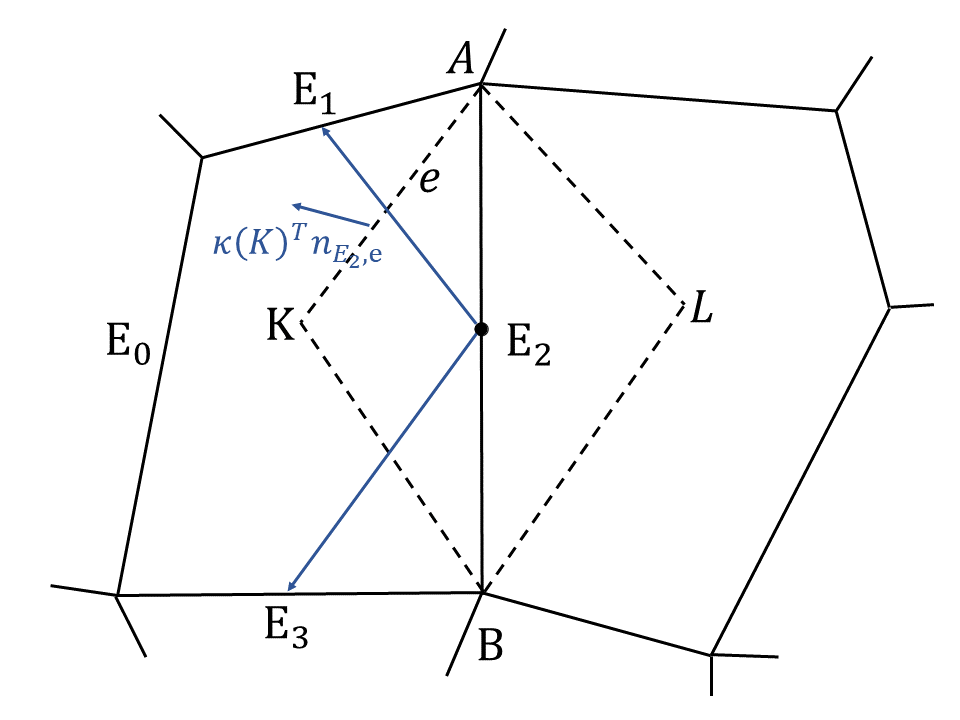
\includegraphics[width=0.5\linewidth]{stencil.png}
\caption{数值格式的模板}
\label{f1}
\end{figure}

我们假设扩散系数在每个单元上近似为常数。$\kappa(x) = \kappa(K) + \mathcal{O}(h)$。得到在虚线网格边上的流量近似为
\begin{equation*}
F_{E, \sigma} = - \int_{\sigma} (\kappa(x) \, \nabla u(x)) \cdot n_{E, \sigma} \ dx = - \nabla u \cdot (|\sigma| \kappa(K)^T \, n_{E, \sigma}) + \mathcal{O}(h^2)
\end{equation*}
向量$|\sigma| \kappa(K)^T n_{E, \sigma}$同样叫做联合法向量。

如图\ref{f1},在单元$K$中,边$E_0,E_1,E_2,E_3$顺时针排列。在计算$E_2$对应的边控制体上的流量时,我们把联合法向量分解成$\overrightarrow{E_2 E_1}, \overrightarrow{E_2 E_3}$的组合,即
\begin{align*}
|\sigma| \kappa(K)^T n_{E_2, \sigma} = \alpha_1 \, \overrightarrow{E_2 E_1} + \alpha_2 \, \overrightarrow{E_2 E_3}
\end{align*}
根据方向导数的性质
\begin{align*}
\nabla u \cdot \overrightarrow{E_2 E_1} = u(E_1) - u(E_2) + \mathcal{O}(h)
\end{align*}
得到流量表示为
\begin{align*}
F_{E_1, \sigma} = (\alpha_{1} \, (u(E_1) - u(E_0)) + \alpha_{2} \, (u(E_1) - u(E_2))) + \mathcal{O}(h^2)
\end{align*}

同理,在相邻的边控制体上,我们也可以得到另一侧的流量$F_{E_2, \sigma}$。既然两个流量都是二阶的,考虑到流守恒的要求,我们可以把两个流平均起来,就得到了最终的流量。(此处要注意符号,$E_1$和$E_2$上计算的流量都是以向外为正方向)
\begin{align*}
F_{\sigma} = \frac12 (F_{E_1, \sigma} - F_{E_2, \sigma})
\end{align*}

这样就得到了最终的数值格式。

\section*{数值实现}

在网格边中点$E$处,它对应的边控制体也用$E$表示。边中点格式表示为
\begin{align*}
\sum_{\sigma} \mathcal{F}_{E, \sigma} = |E| \, f(E)
\end{align*}
注意,这里的$f(E)$表示的是右端项在四边形控制体内的积分平均,而不是在边中点处的函数值。

在程序中,我们要遍历每条单元中心和节点之间的连线来装配总体的系数矩阵。

设单元$U$中,对应的边为$E_0, E_1, \cdots E_n$,按顺时针排列。节点$P$位于$E_1, E_2$之间。$\sigma = U P$是单元中心和节点的连线。它的法向为$n_e$,从$E_1$指向$E_2$。

在$E_1$对应的边控制体上,$\sigma$上沿着$n_e$方向的流量为
\begin{align*}
F_{E_1, \sigma} = \alpha_{1,0} \, (u(E_1) - u(E_0)) + \alpha_{1,2} \, (u(E_1) - u(E_2))
\end{align*}
其中系数由向量分解确定
\begin{align*}
|\sigma| \kappa(K)^T n_{\sigma} = \alpha_{1,0} \, \overrightarrow{E_1 E_0} + \alpha_{1,2} \, \overrightarrow{E_1 E_2}
\end{align*}

在$E_2$对应的边控制体上,$\sigma$上沿着$n_e$方向的流量为
\begin{align*}
F_{E_2, \sigma} = \alpha_{2,1} \, (u(E_2) - u(E_1)) + \alpha_{2,3} \, (u(E_2) - u(E_3))
\end{align*}
其中系数由向量分解确定
\begin{align*}
|\sigma| \kappa(K)^T n_{\sigma} = \alpha_{2,1} \, \overrightarrow{E_2 E_1} + \alpha_{2,3} \, \overrightarrow{E_2 E_3}
\end{align*}

平均之后的流量为
\begin{align*}
F_{\sigma} = \frac12 F_{E_1, \sigma} + \frac12 F_{E_2, \sigma}
\end{align*}

计算边$\sigma$上的流量时,相当于把这两个边流量矩阵加到总体矩阵中去
\begin{align*}
\frac12
\left(
\begin{matrix}
-\alpha_{1,0} & \alpha_{1,0} + \alpha_{1,2} & - \alpha_{1,2} \\
\alpha_{1,0} & -\alpha_{1,0} - \alpha_{1,2} & \alpha_{1,2} 
\end{matrix}
\right)
\end{align*}
在总体矩阵中对应第$E_1, E_2$行和第$E_0, E_1, E_2$列,
\begin{align*}
\frac12
\left(
\begin{matrix}
-\alpha_{2,1} & \alpha_{2,1} + \alpha_{2,3} & - \alpha_{2,3} \\
\alpha_{2,1} & -\alpha_{2,1} - \alpha_{2,3} & \alpha_{2,3} 
\end{matrix}
\right)
\end{align*}
在总体矩阵中对应第$E_1, E_2$行和第$E_1, E_2, E_3$列,


只考虑Dirichlet边界条件。如果某条边$E_i$在区域边界,它直接通过方程的边界条件得到。就是在矩阵中$E_i$对应的行全部改成0,只有第$E_i$行,第$E_i$列为$1$,右端项中$E_i$对应的位置为边界条件在$E_i$处的值。


\section*{实验结果}

\subsection*{实验1}

求解稳态扩散方程,精确解和扩散系数选为
\begin{align*}
u = \sin((x-1)(y-1)) - (x-1)^3 (y-1)^2 \qquad
a = \left[
\begin{matrix}
1.5 & 0.5 \\
0.5 & 1.5 \\
\end{matrix}
\right]
\end{align*}
网格为随机多边形网格,使用的网格和结果如图。

\begin{figure}[H]
\centering
\subfloat[多边形网格]{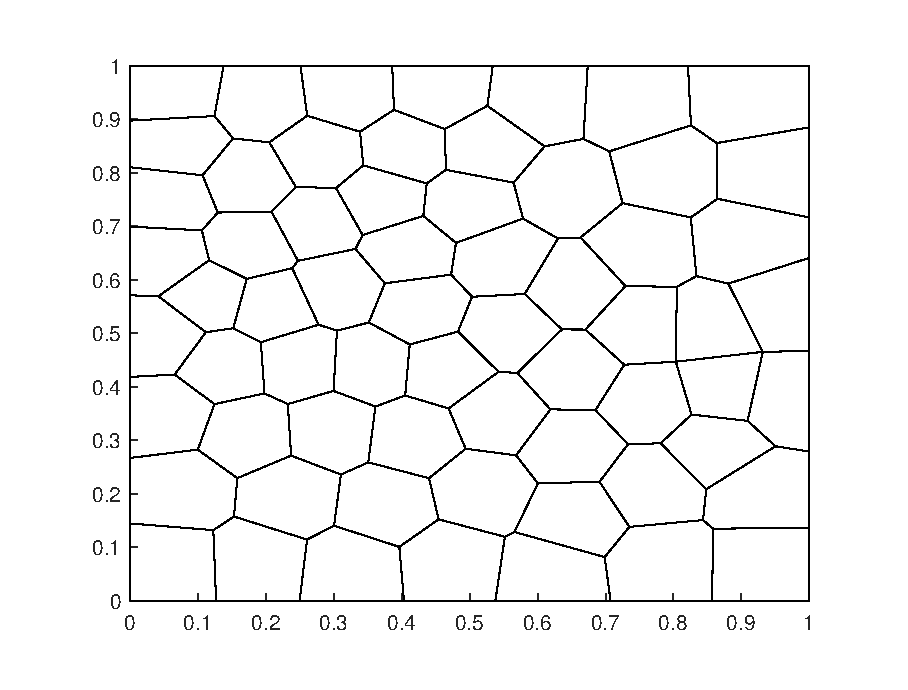
\includegraphics[width=0.3\linewidth]{mesh1}}
\subfloat[数值解$u_h$]{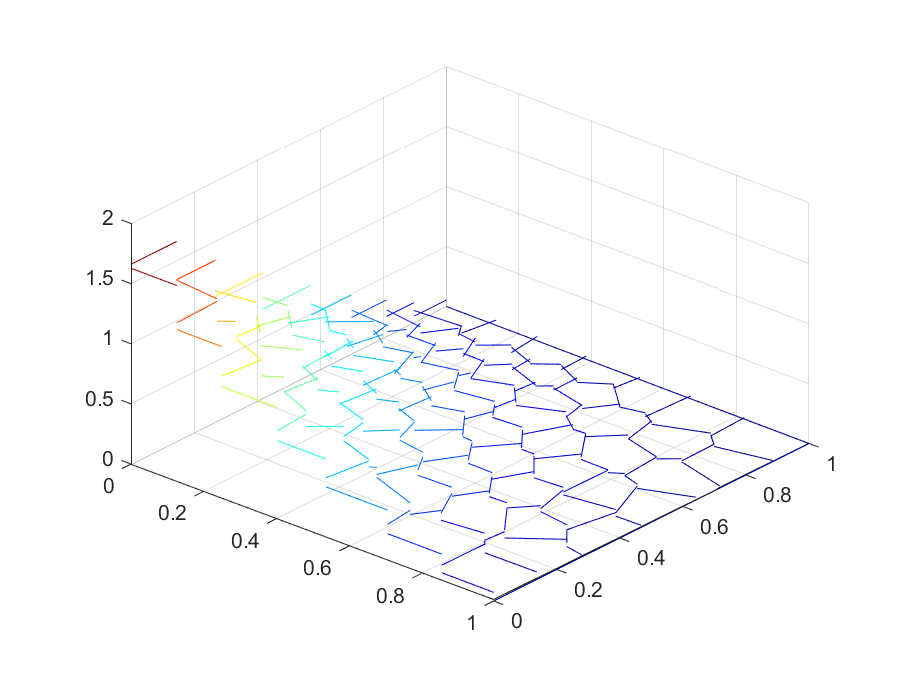
\includegraphics[width=0.3\linewidth]{u1}}
\subfloat[误差$u - u_h$]{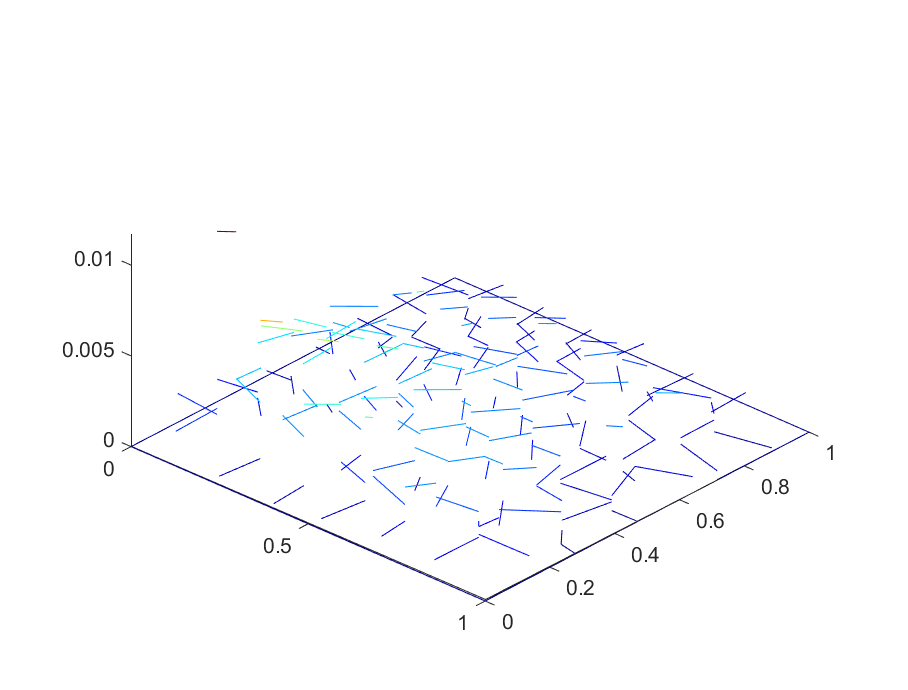
\includegraphics[width=0.3\linewidth]{e1}}
\caption{实验结果1}
\end{figure}

在这样的网格上,误差已经达到了$10^{-2}$。

\subsection*{实验2}

精确解和扩散系数选为
\begin{align*}
u = 16 \, x \, y \, (1-x) \, (1-y) \qquad
a = \left[
\begin{matrix}
1.5 & 0.5 \\
0.5 & 1.5 \\
\end{matrix}
\right]
\end{align*}
使用的网格如图。对网格不断加密,得到收敛阶如下表
\begin{figure}[H]
\centering
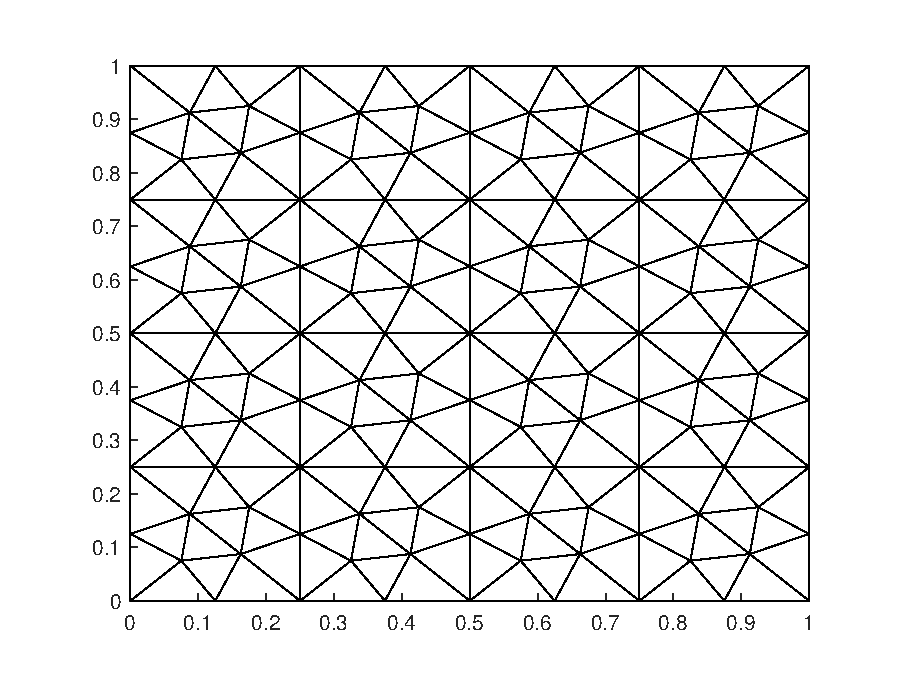
\includegraphics[width=0.4\linewidth]{mesh2}
\caption{实验2网格}
\end{figure}

\begin{table}
\centering
\begin{tabular}{ccc|ccc}
\multicolumn{3}{c}{九点有限体积格式}  & \multicolumn{3}{c}{边中点有限体积格式} \\
\hline
DOF & $\|u - u_h\|_{\infty}$ & order & DOF & $\|u - u_h\|_{\infty}$ & order \\
\hline
56 & 4.32e-02 & * & 92 & 5.43e-02 & * \\
224 & 1.08e-02 & 1.99381 & 352 & 1.77e-02 & 1.67478 \\
896 & 2.72e-03 & 1.99582 & 1376 & 4.96e-03 & 1.86234 \\
3584 & 6.81e-04 & 1.99781 & 5440 & 1.31e-03 & 1.93628 \\
14336 & 1.70e-04 & 1.99893 & 21632 & 3.37e-04 & 1.9693 \\
\hline
\end{tabular}
\end{table}

边中点有限体积格式可以达到二阶收敛,而且在某些特殊的网格上,它比九点格式更有优势。

%\bibliographystyle{plain}
%\bibliography{FVM}

\end{document}